\documentclass{article}
\usepackage{gensymb, amsmath, float, graphicx, epstopdf}
\restylefloat{table}
\usepackage[margin=0.75in]{geometry}
\begin{document}

\title{Lab Write-up 2: The Smith Chart}
\author{Michael Shen}
\maketitle

\section{Line Parameters of a Lossless Line}
\subsection{Measured Data}
\begin{table}[h]
\centering
	\begin{tabular}{rl}
	Patch Cord Length =  	  & 0.6229 $m$  \\
	Added Electrical Delay =  & 0.16806 $ns$      
	\end{tabular}
\end{table}
\subsection{Analysis}
\begin{enumerate}
	\item 
		\begin{equation}
			u_p = \dfrac{2l}{\Delta t}
		\end{equation}
		Using the measured data and Eq. 1, the calculated $u_p$ is 
	\item
	\item
	\item
\end{enumerate}
\subsection{Questions}
\begin{enumerate}
	\item
	\item
	\item
	\item
\end{enumerate}

\section{Lossy and Lossless Lines on the Smith Chart}
\subsection{Analysis}
\begin{enumerate}
	\item
	\item
\end{enumerate}
\subsection{Questions}
\begin{enumerate}
	\item
\end{enumerate}
\section{Impedance Measurements Using the Smith Chart}
\subsection{Measured Data}
\begin{table}[h]
\centering
	\begin{tabular}{rl}
	Resistor =   & 2212 $\Omega$  \\
	Capacitor =  & 1808 $pF$      
	\end{tabular}
\end{table}

\begin{table}[H]
\centering
	\begin{tabular}{|c|c|c|c|c|c|}
	\hline
	\textbf{Frequency} & \textbf{Cable} & $v_1$ (V) & $v_2$ (V) & $\Delta$T (ns) & $\Delta\varphi\degree$ \\ \hline
	$f_{1}$ = 100 kHz  & 12"                & 5.65   & 2.55   & -16     & -0.5      \\ \hline
	                   & 180"               & 5.85   & 2.55   & 60      & 2.7       \\ \hline
	$f_{2}$ = 100 MHz  & 12"                & 4.35   & 0.133  & 1.48    & 50        \\ \hline
	                   & 180"               & 3.35   & 0.116  & 1.48    & 50        \\ \hline
	\end{tabular}
	\caption{Voltage and phase measurements for varying signal frequency and cable length}
	\label{Data 1}
\end{table}
\subsection{Analysis}
\begin{enumerate}
	\item
	\item
	\item
	\item
\end{enumerate}
\subsection{Questions}
\begin{enumerate}
	\item
	\item
\end{enumerate}
\section{Impedance Matching Using a Single Stub Tuner}
\subsection{Measured Data}
\begin{table}[h]
\centering
	\begin{tabular}{rl}
	Impedance before Matching =   			 & 2212 $\Omega$  \\
	Distance between Load and Stub Tuner =   & 2212 $cm$  \\
	Length of Stub =   						 & 2212 $cm$  \\
	Impedance after Matching =  			 & 1808 $\Omega$      
	\end{tabular}
\end{table}
\subsection{Analysis}
\begin{enumerate}
	\item
	\item
	\item
\end{enumerate}
\subsection{Questions}
\begin{enumerate}
	\item
	\item
	\item
\end{enumerate}

\section{Figures and Images}
\begin{figure}[H]
    \centering
    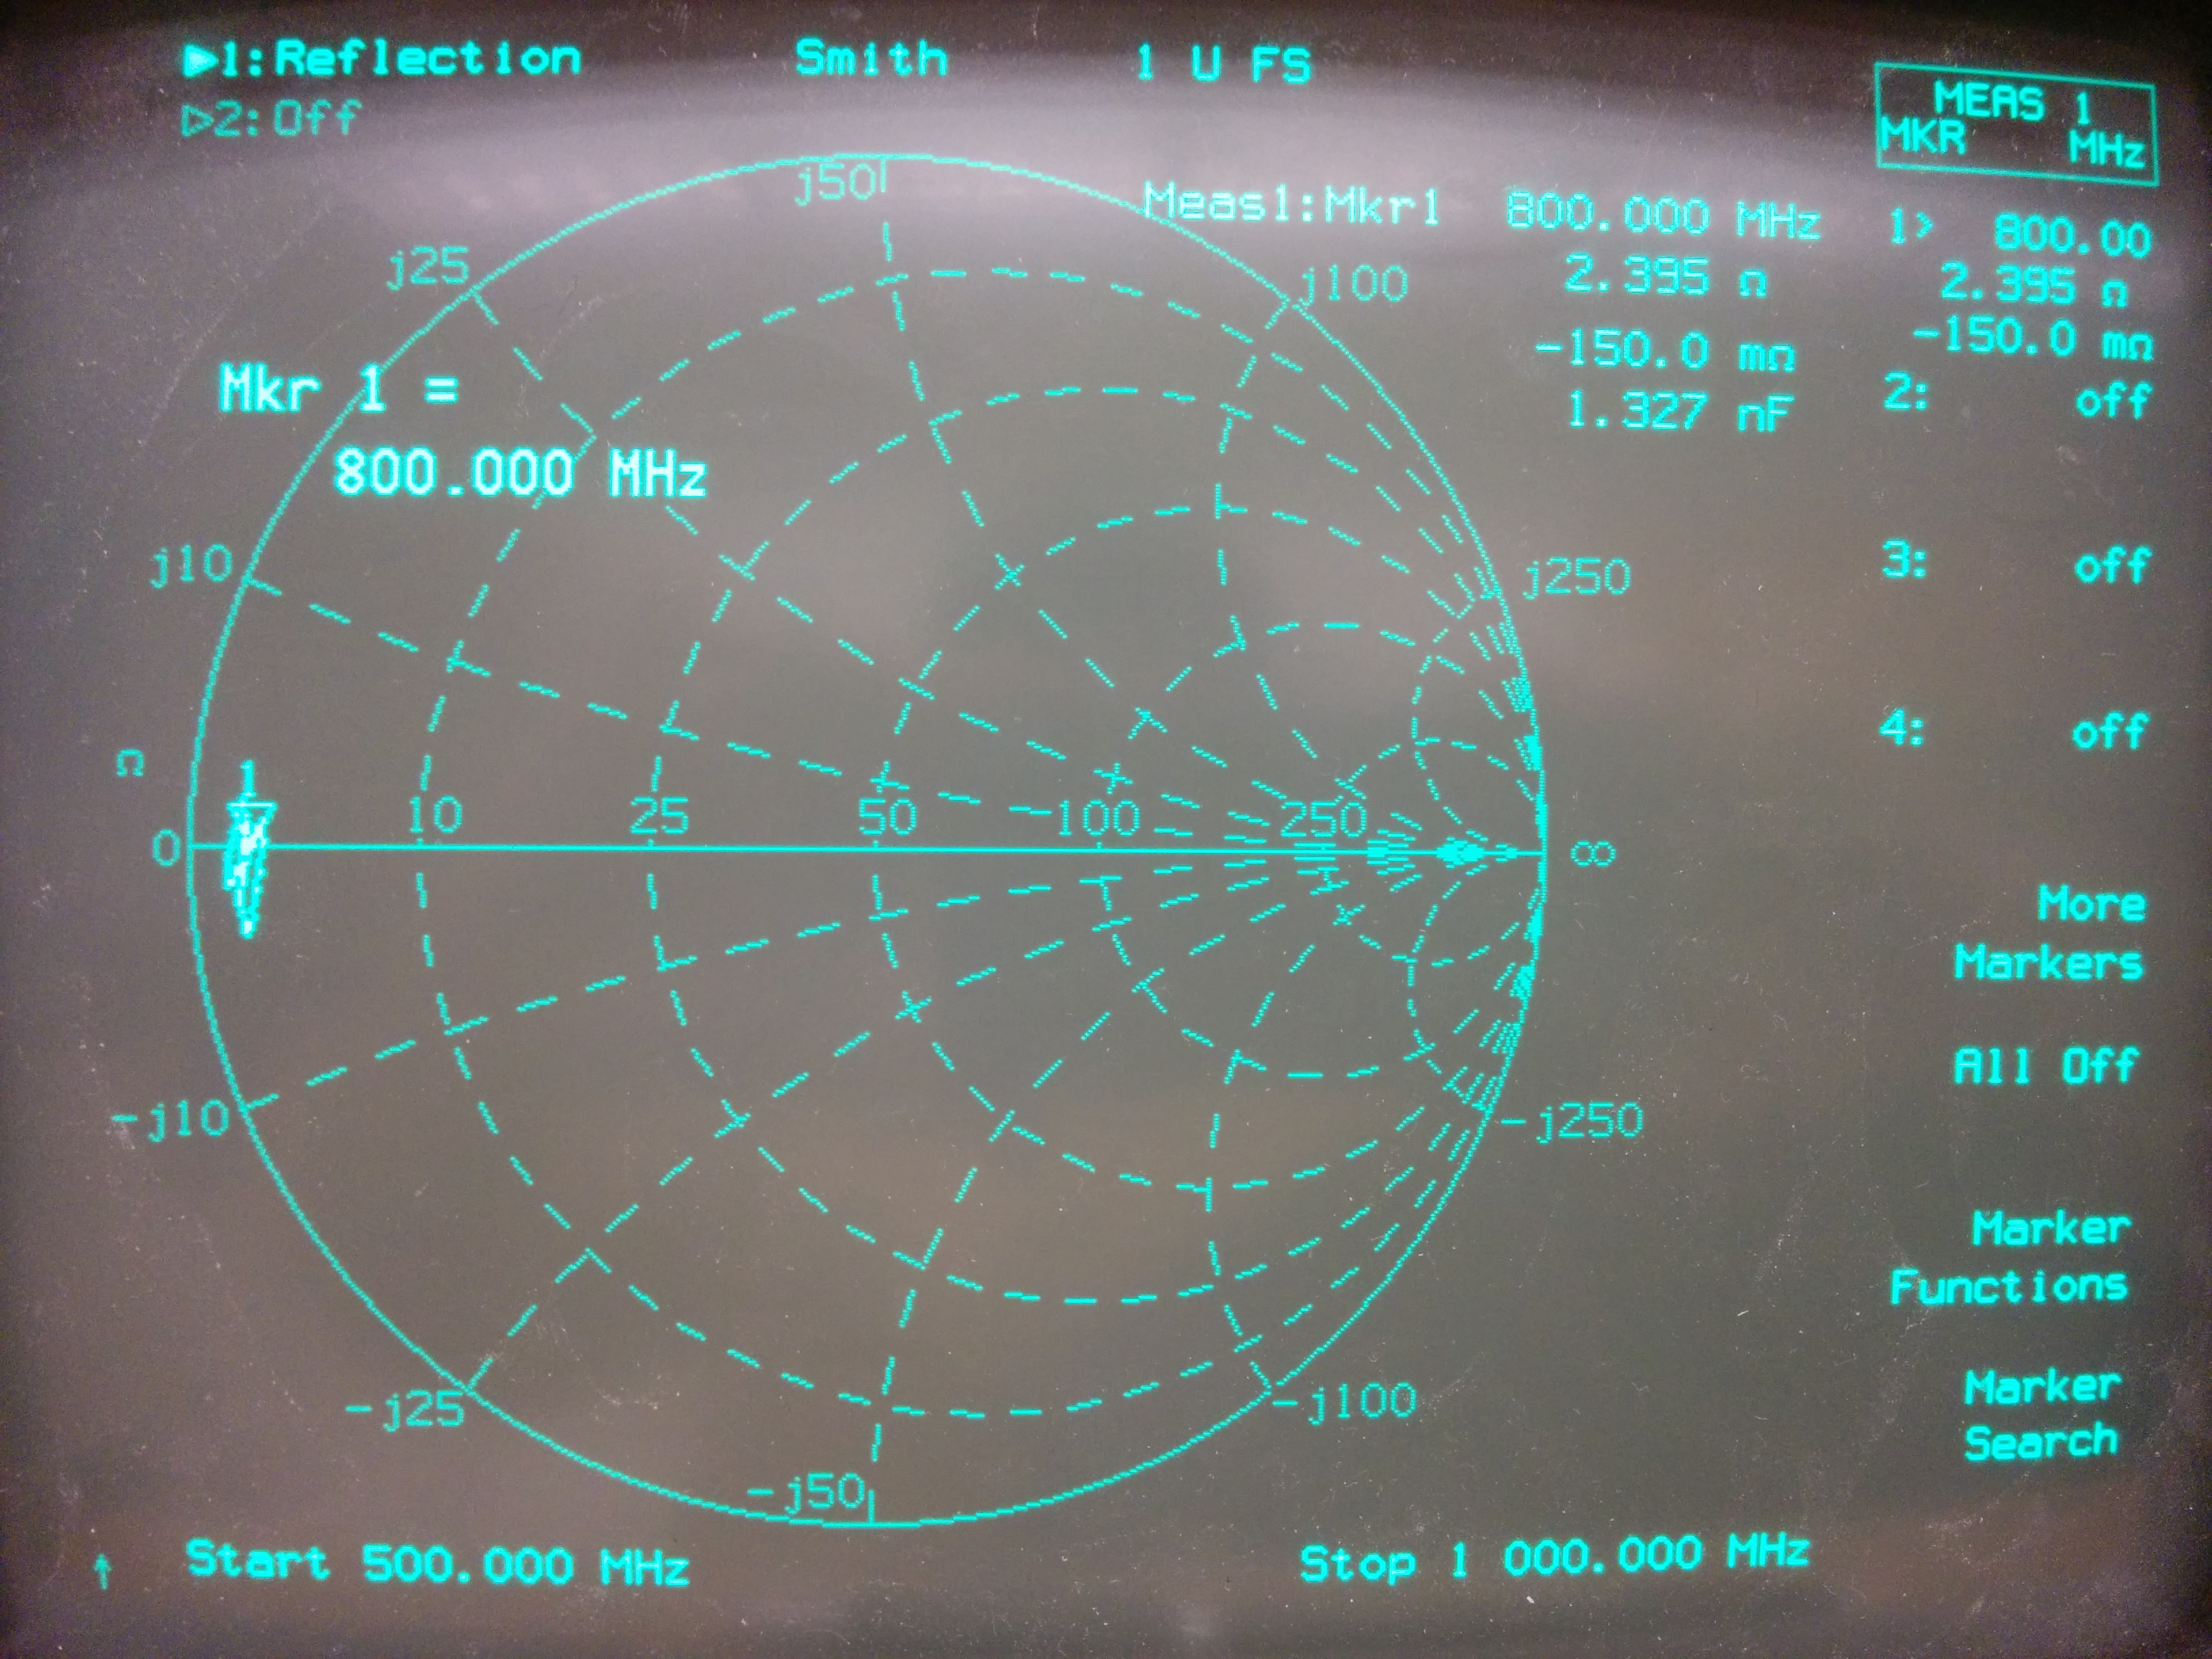
\includegraphics[width=0.8\textwidth]{./Images/251.jpg}
    \caption{Point-like response for a lossless line}
\end{figure}
\begin{figure}[H]
    \centering
    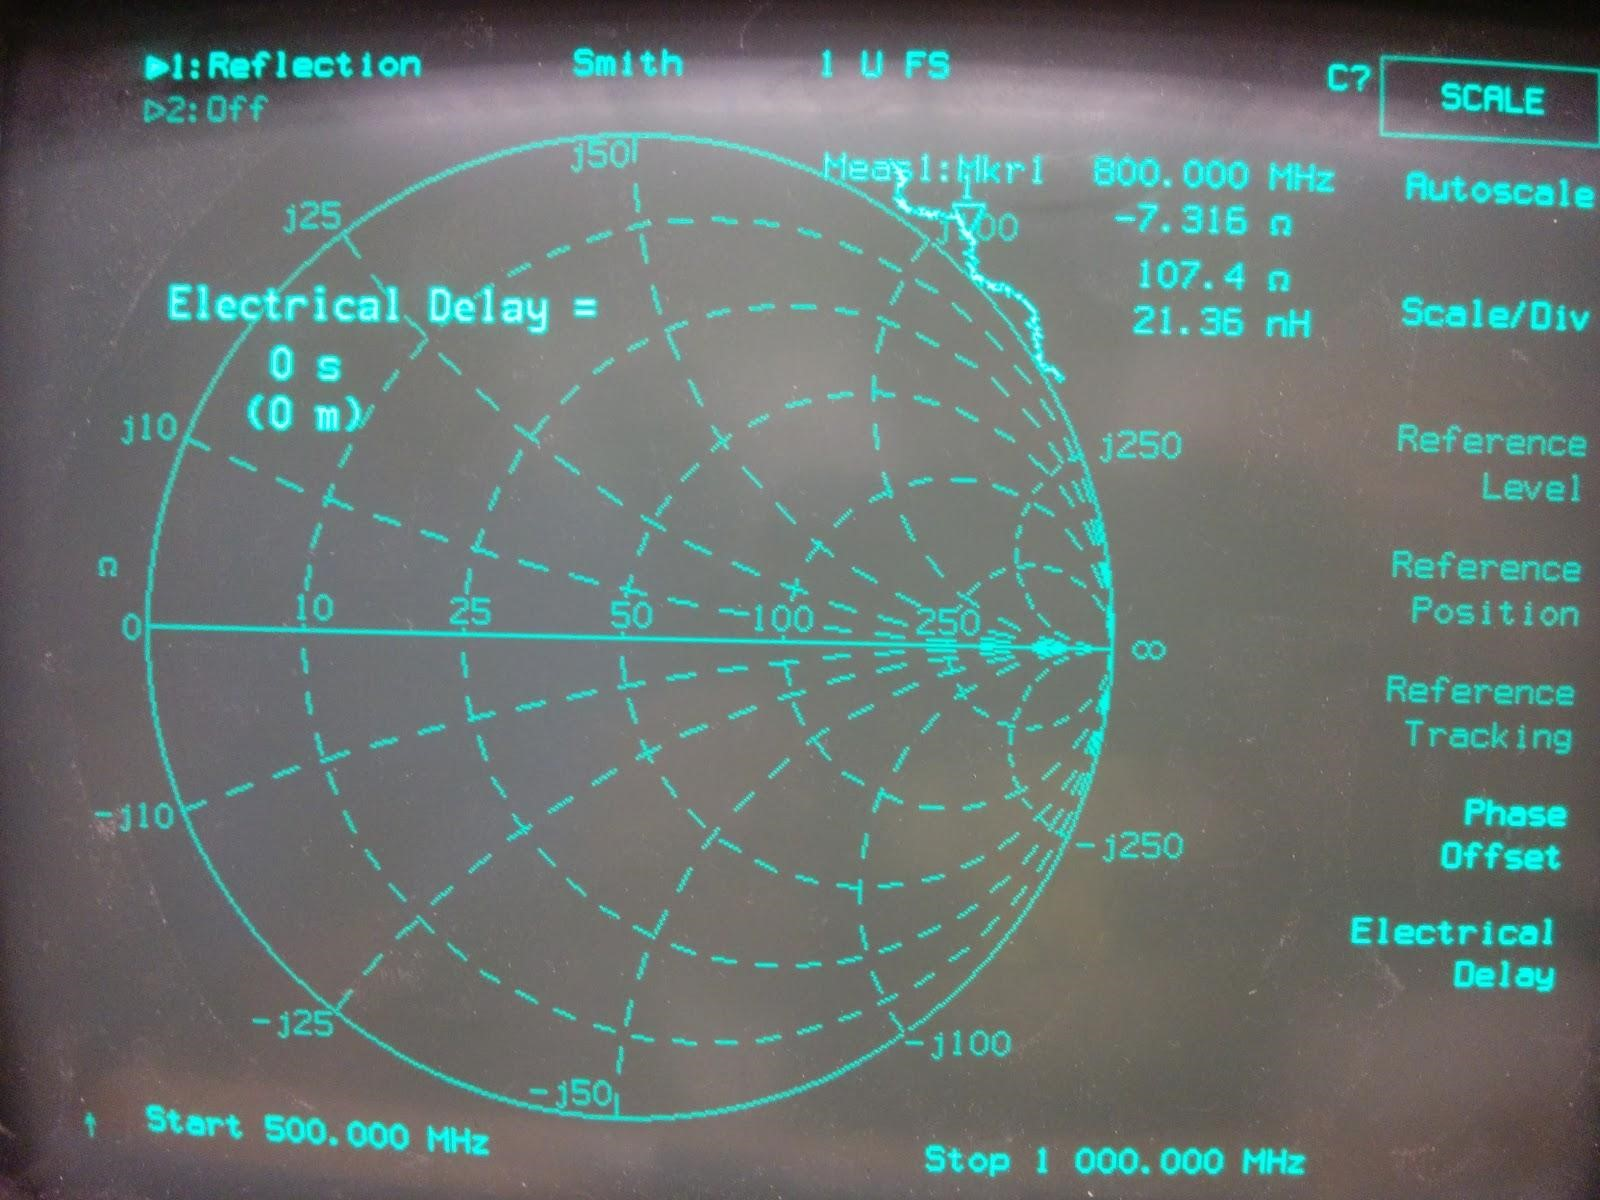
\includegraphics[width=0.8\textwidth]{./Images/252lossless.jpg}
    \caption{Network Analyzer response for a lossless line}
\end{figure}
\begin{figure}[H]
    \centering
    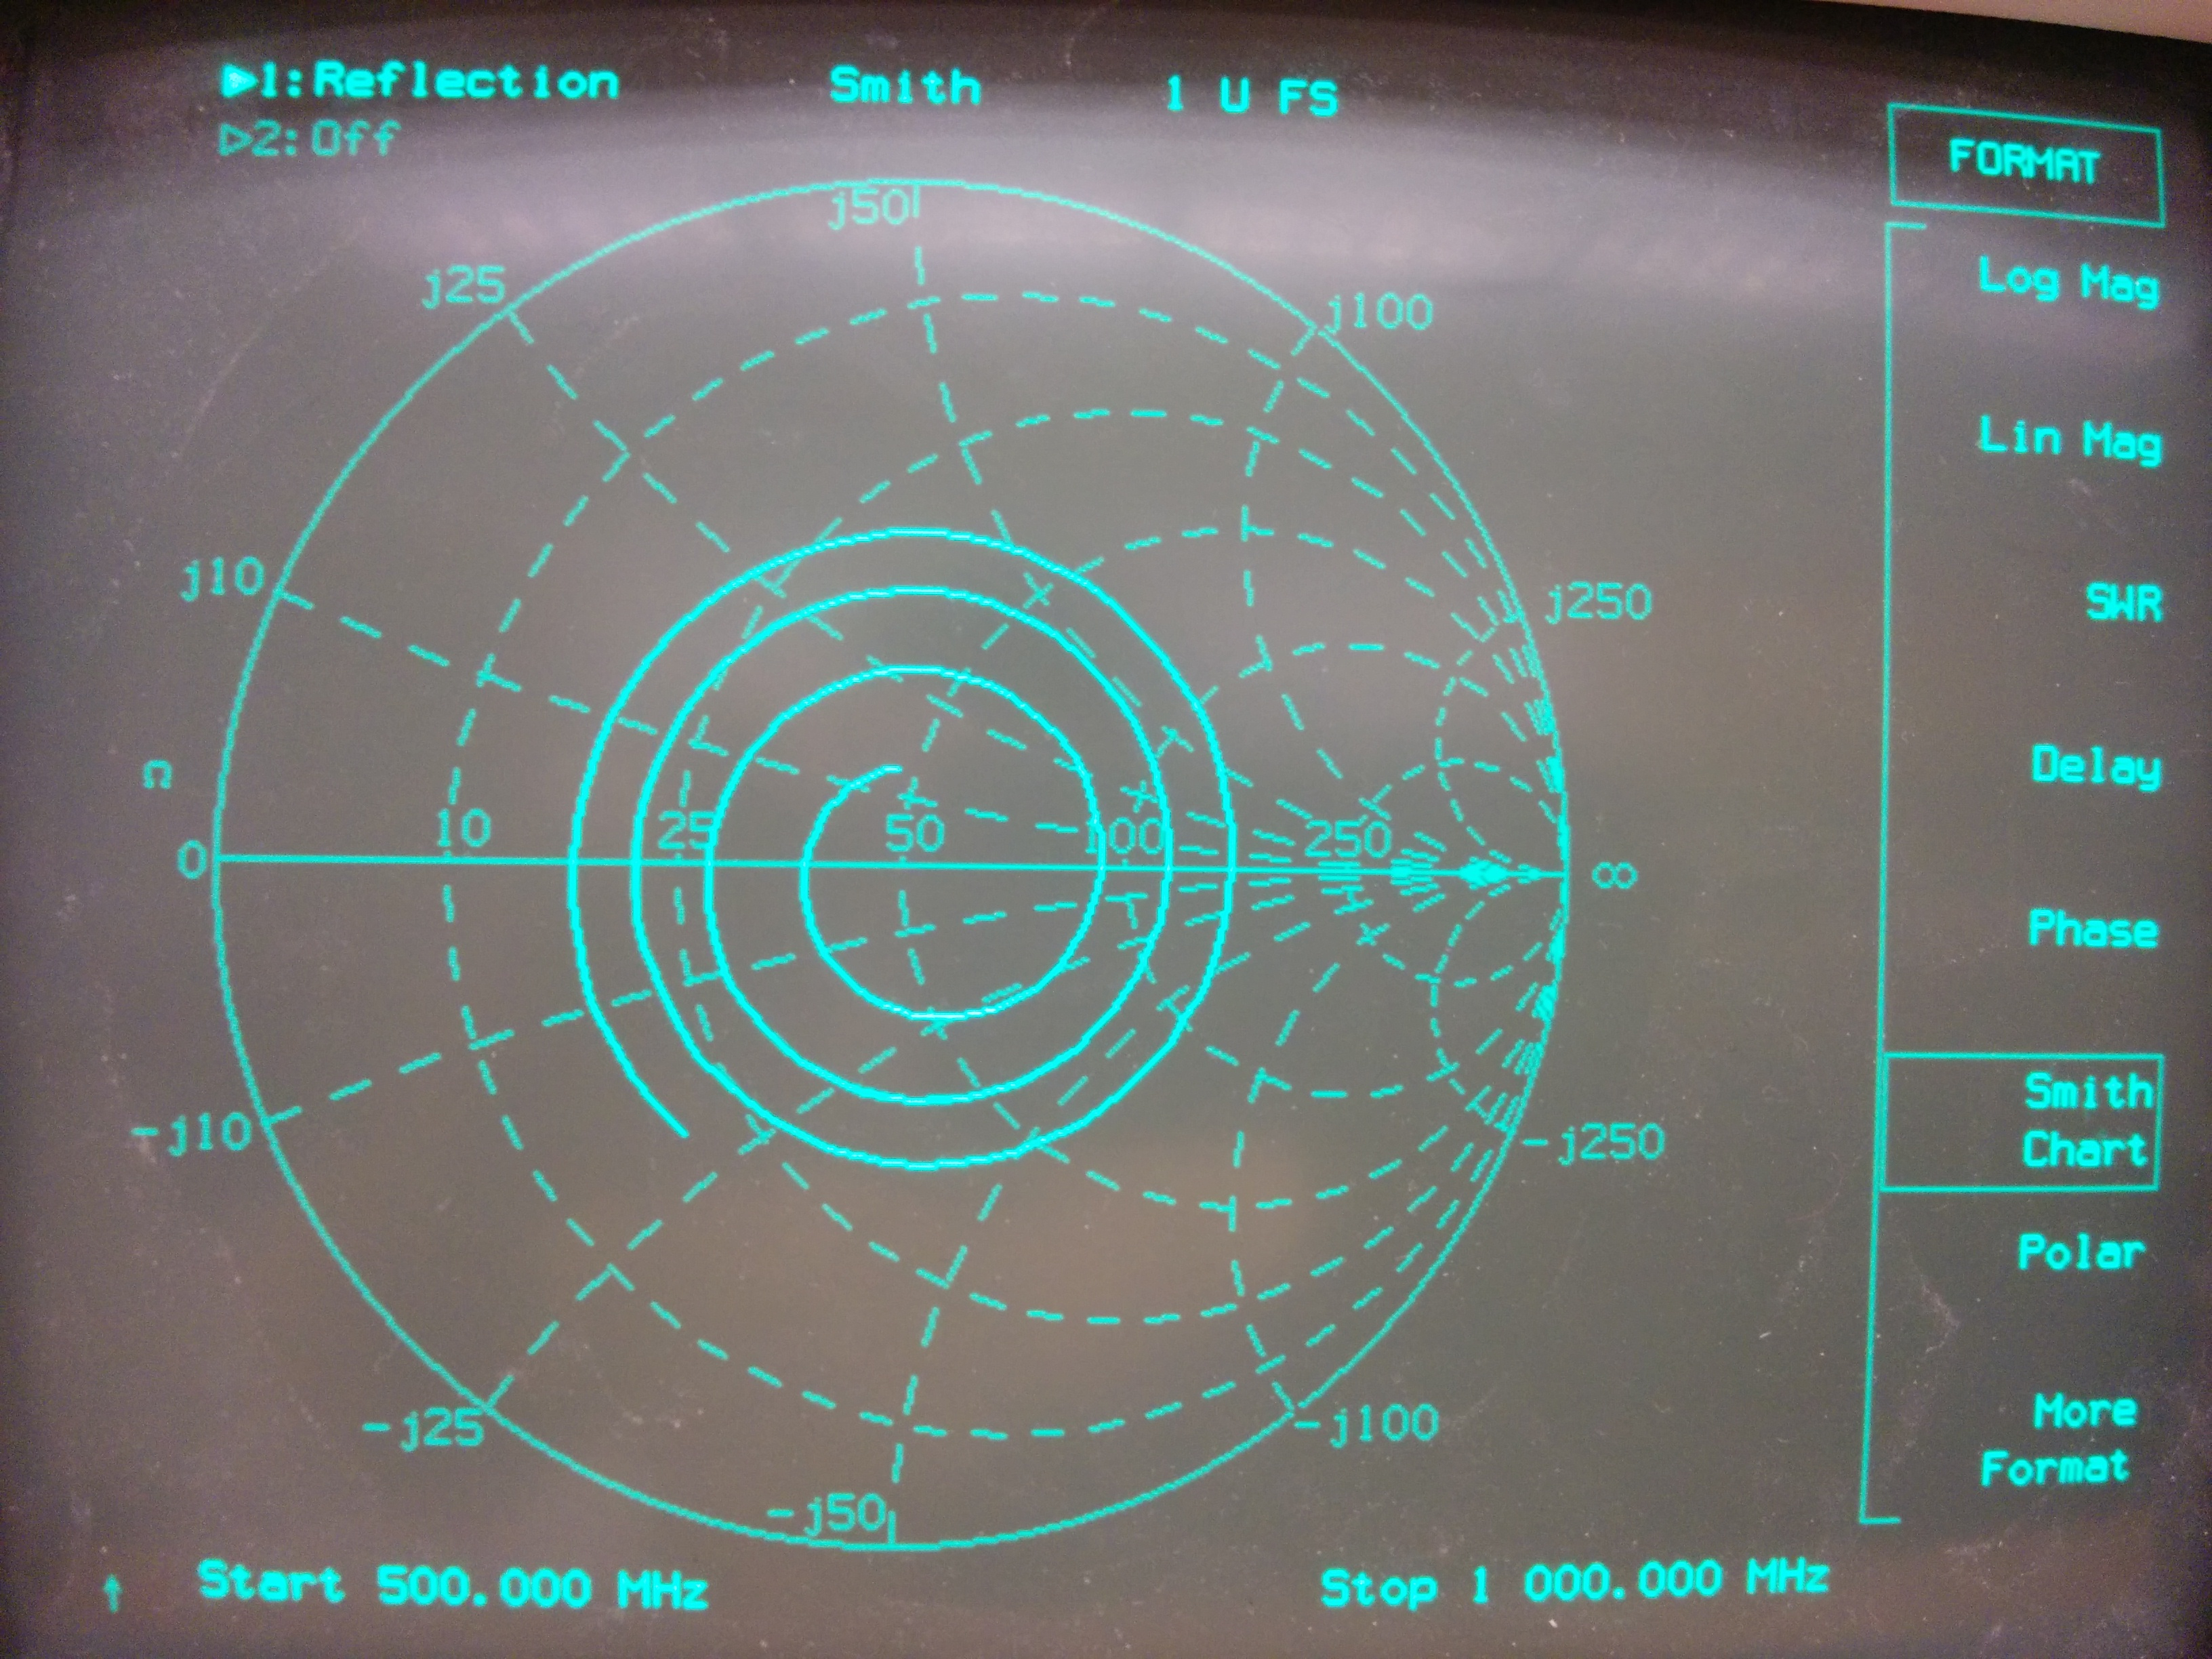
\includegraphics[width=0.8\textwidth]{./Images/252lossy.jpg}
    \caption{Network Analyzer response for a lossy line}
\end{figure}
\begin{figure}[H]
    \centering
    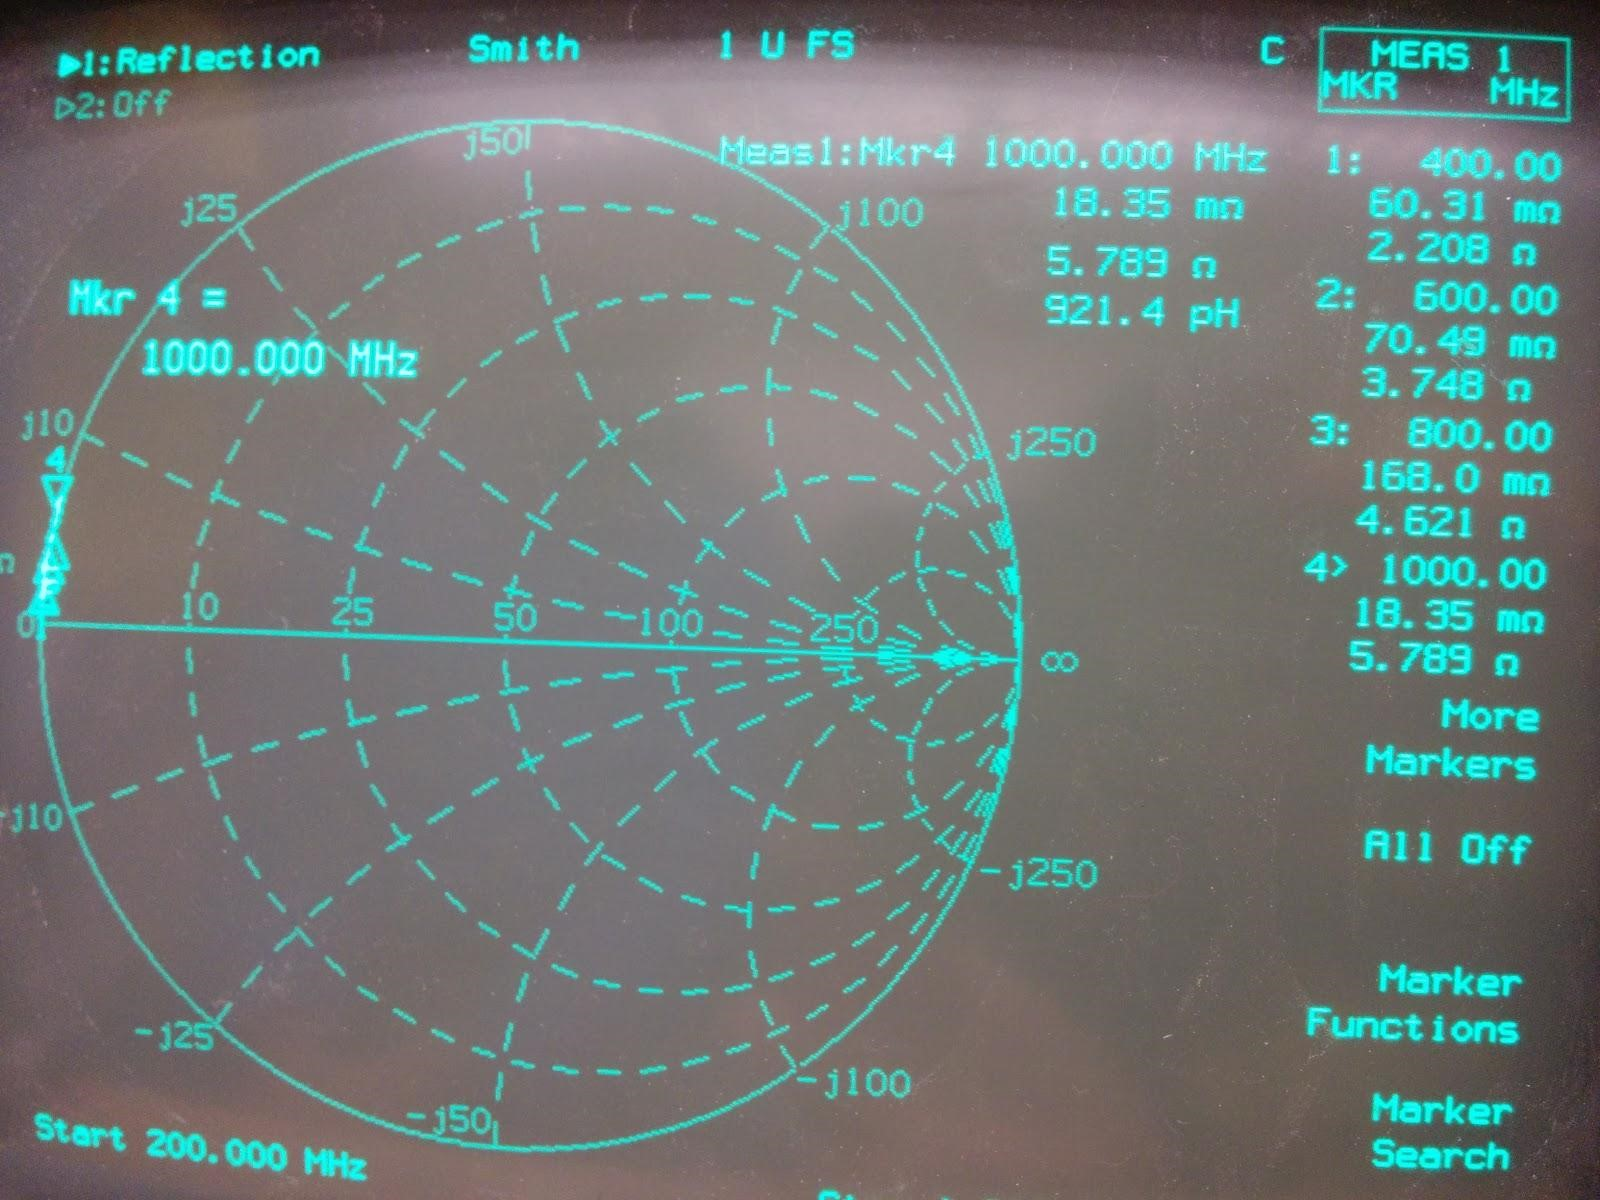
\includegraphics[width=0.8\textwidth]{./Images/253short.jpg}
    \caption{Network Analyzer response for a shorted load}
\end{figure}
\begin{figure}[H]
    \centering
    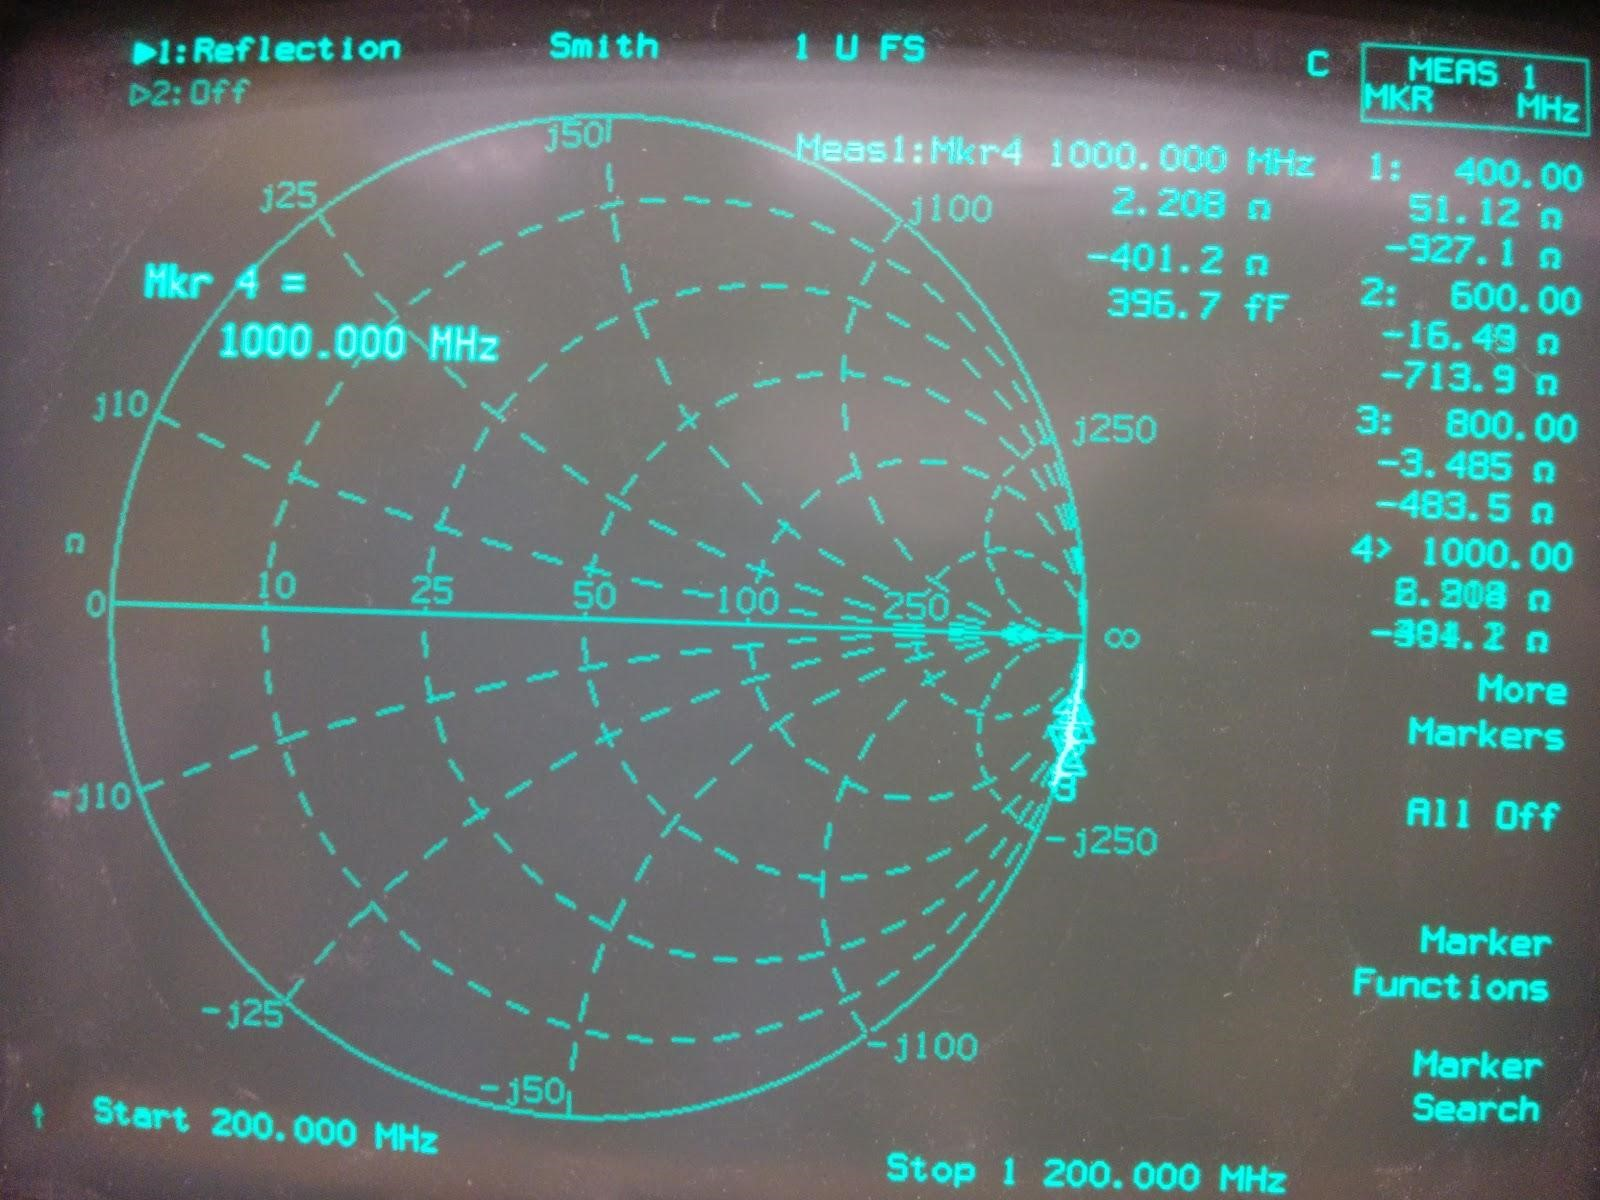
\includegraphics[width=0.8\textwidth]{./Images/253open.jpg}
    \caption{Network Analyzer response for an open load}
\end{figure}
\begin{figure}[H]
    \centering
    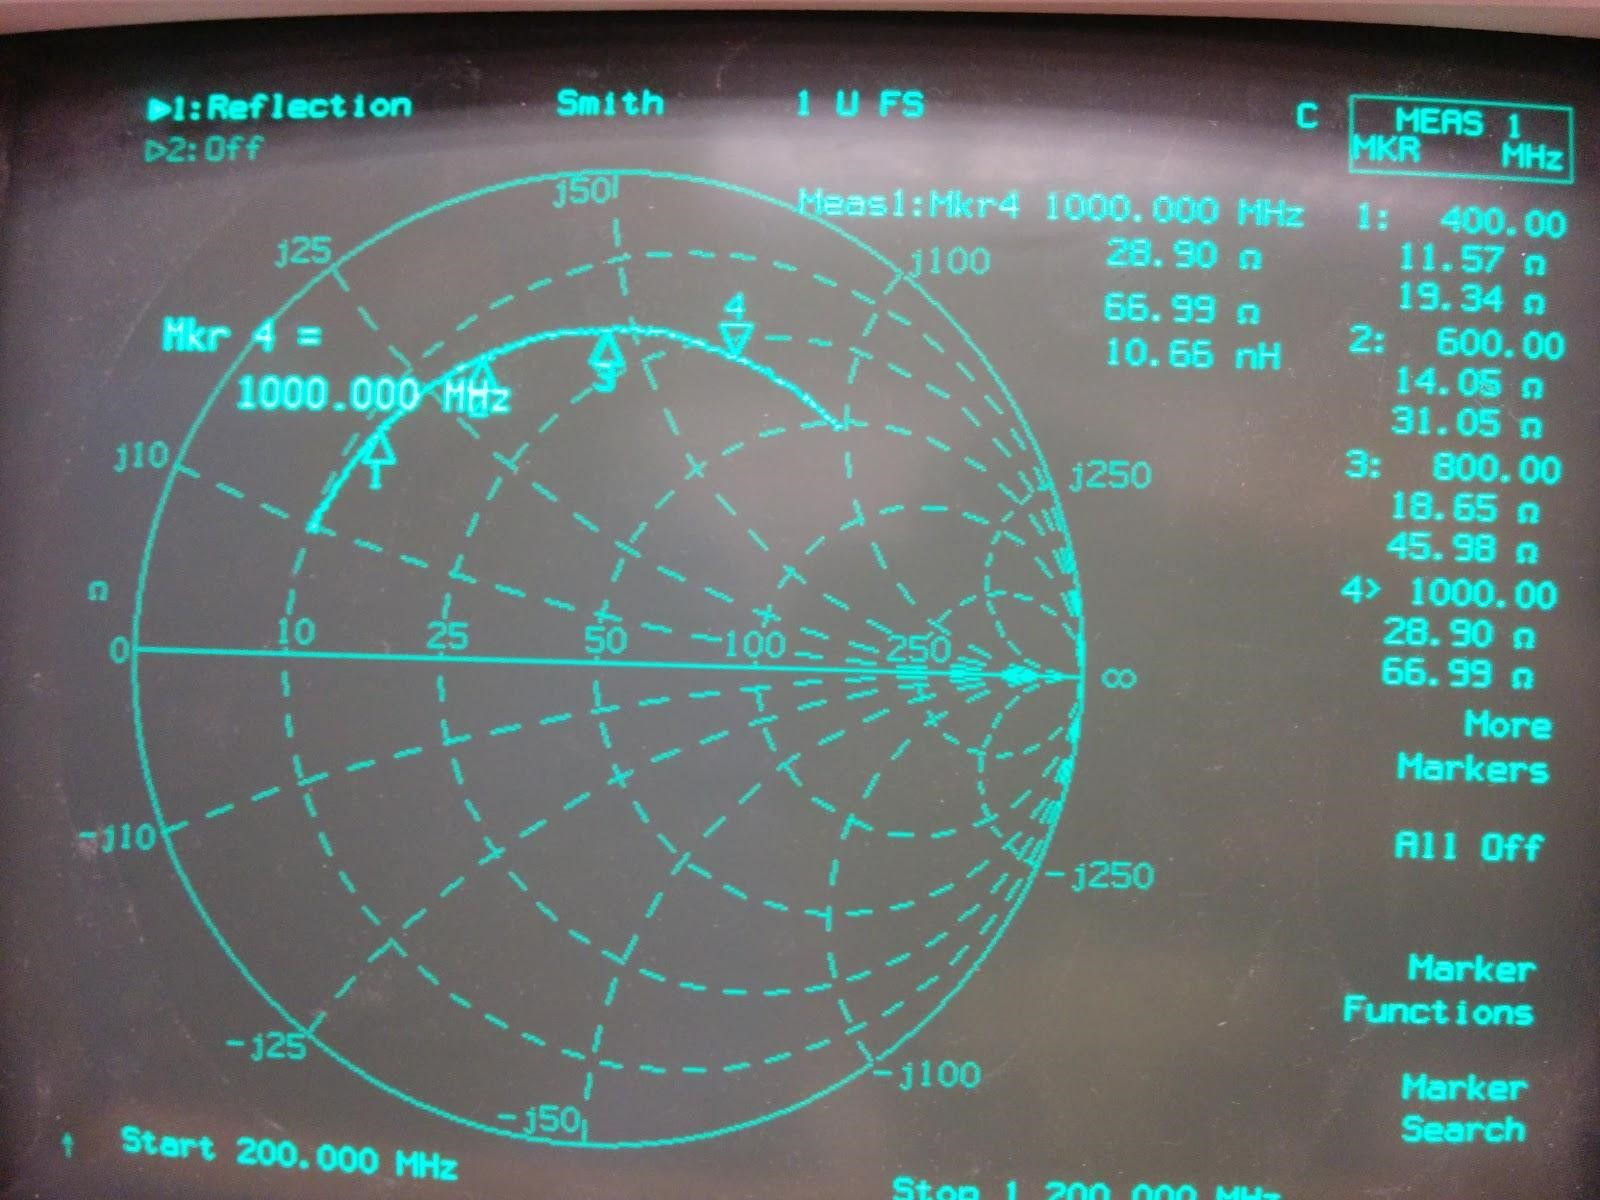
\includegraphics[width=0.8\textwidth]{./Images/253resisitive.jpg}
    \caption{Network Analyzer response for a resistive load}
\end{figure}
\begin{figure}[H]
    \centering
    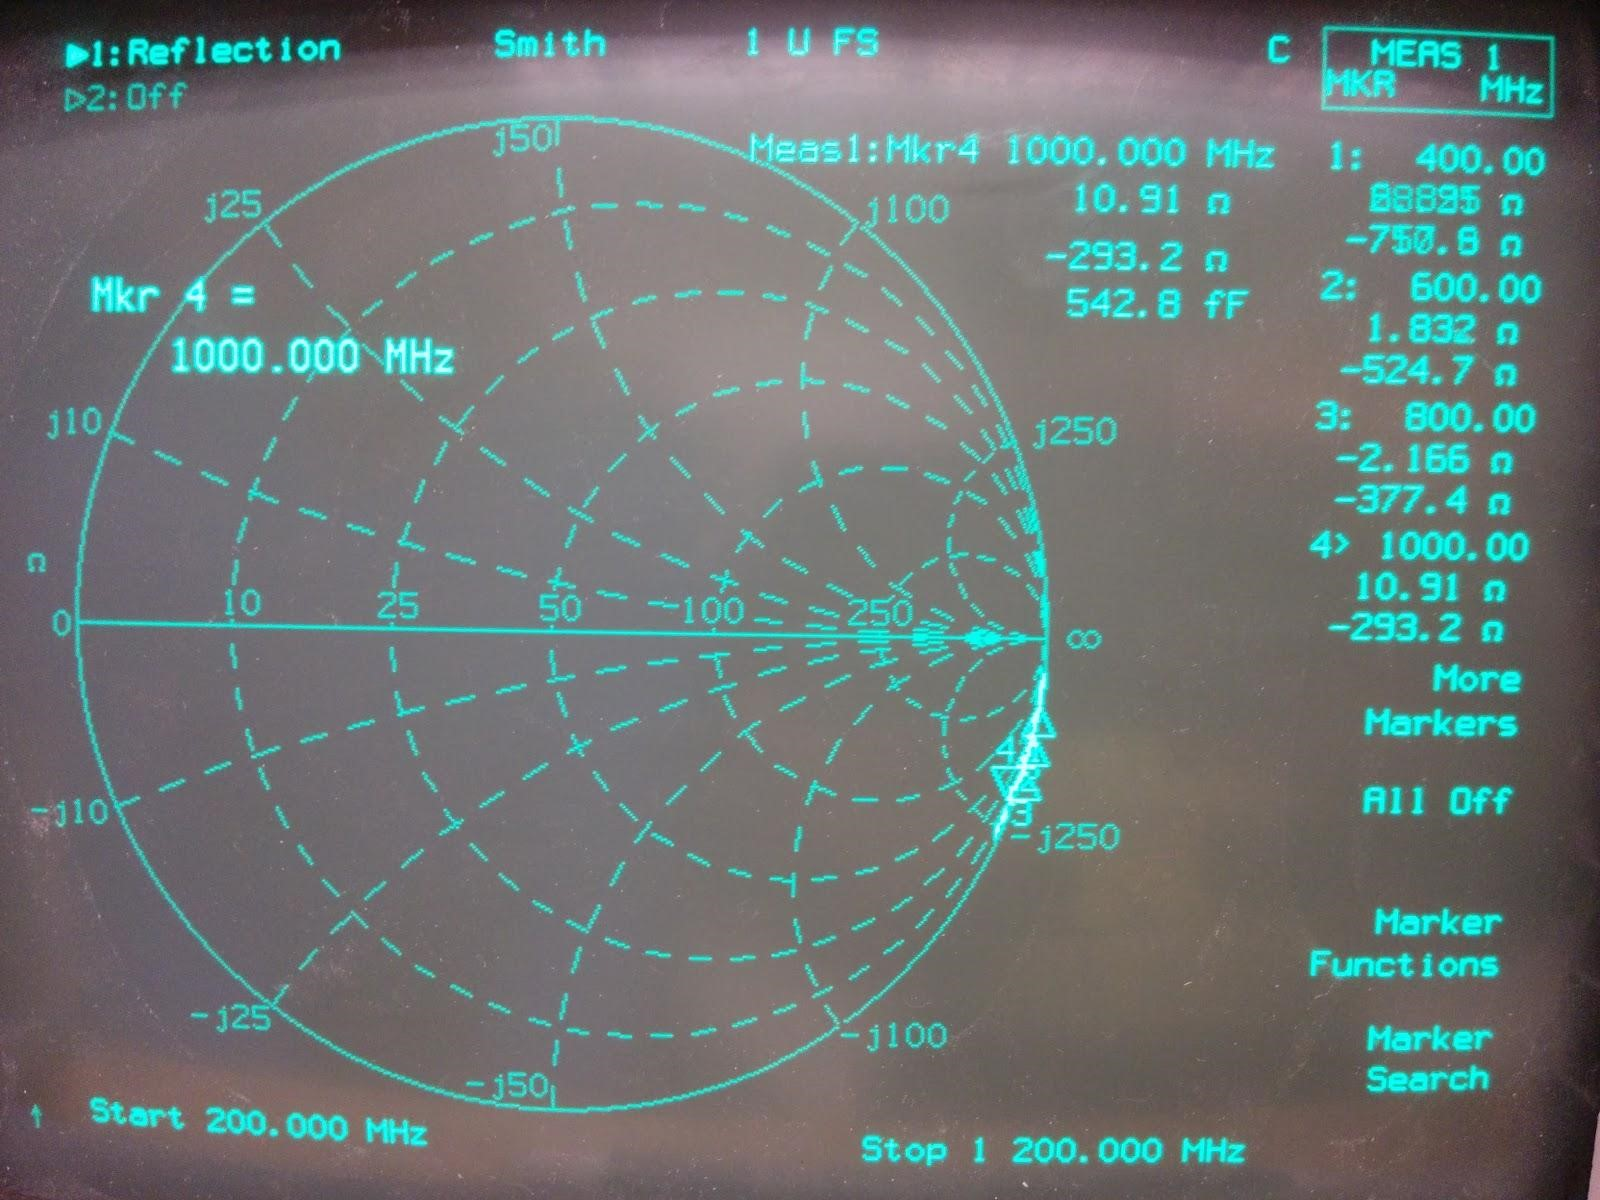
\includegraphics[width=0.8\textwidth]{./Images/253capacitive.jpg}
    \caption{Network Analyzer response for a capacitive load}
\end{figure}
\begin{figure}[H]
    \centering
    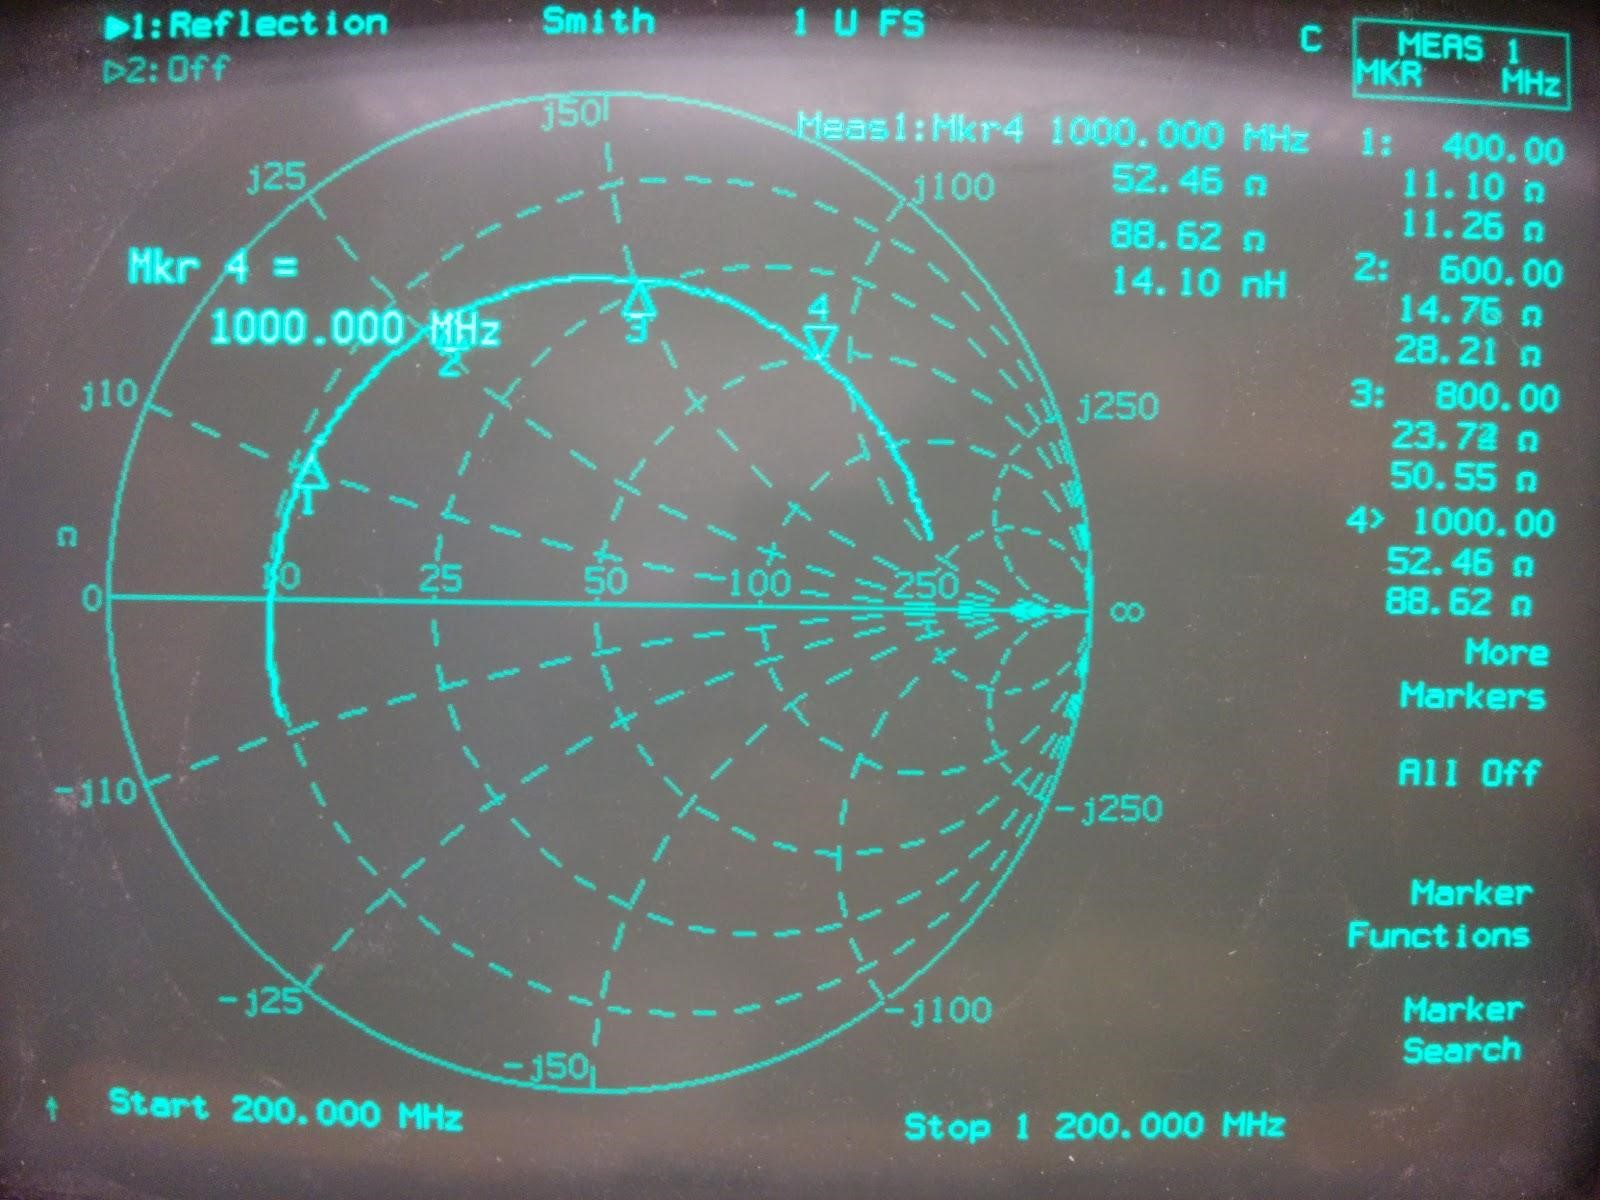
\includegraphics[width=0.8\textwidth]{./Images/253series.jpg}
    \caption{Network Analyzer response for a series load}
\end{figure}
\begin{figure}[H]
    \centering
    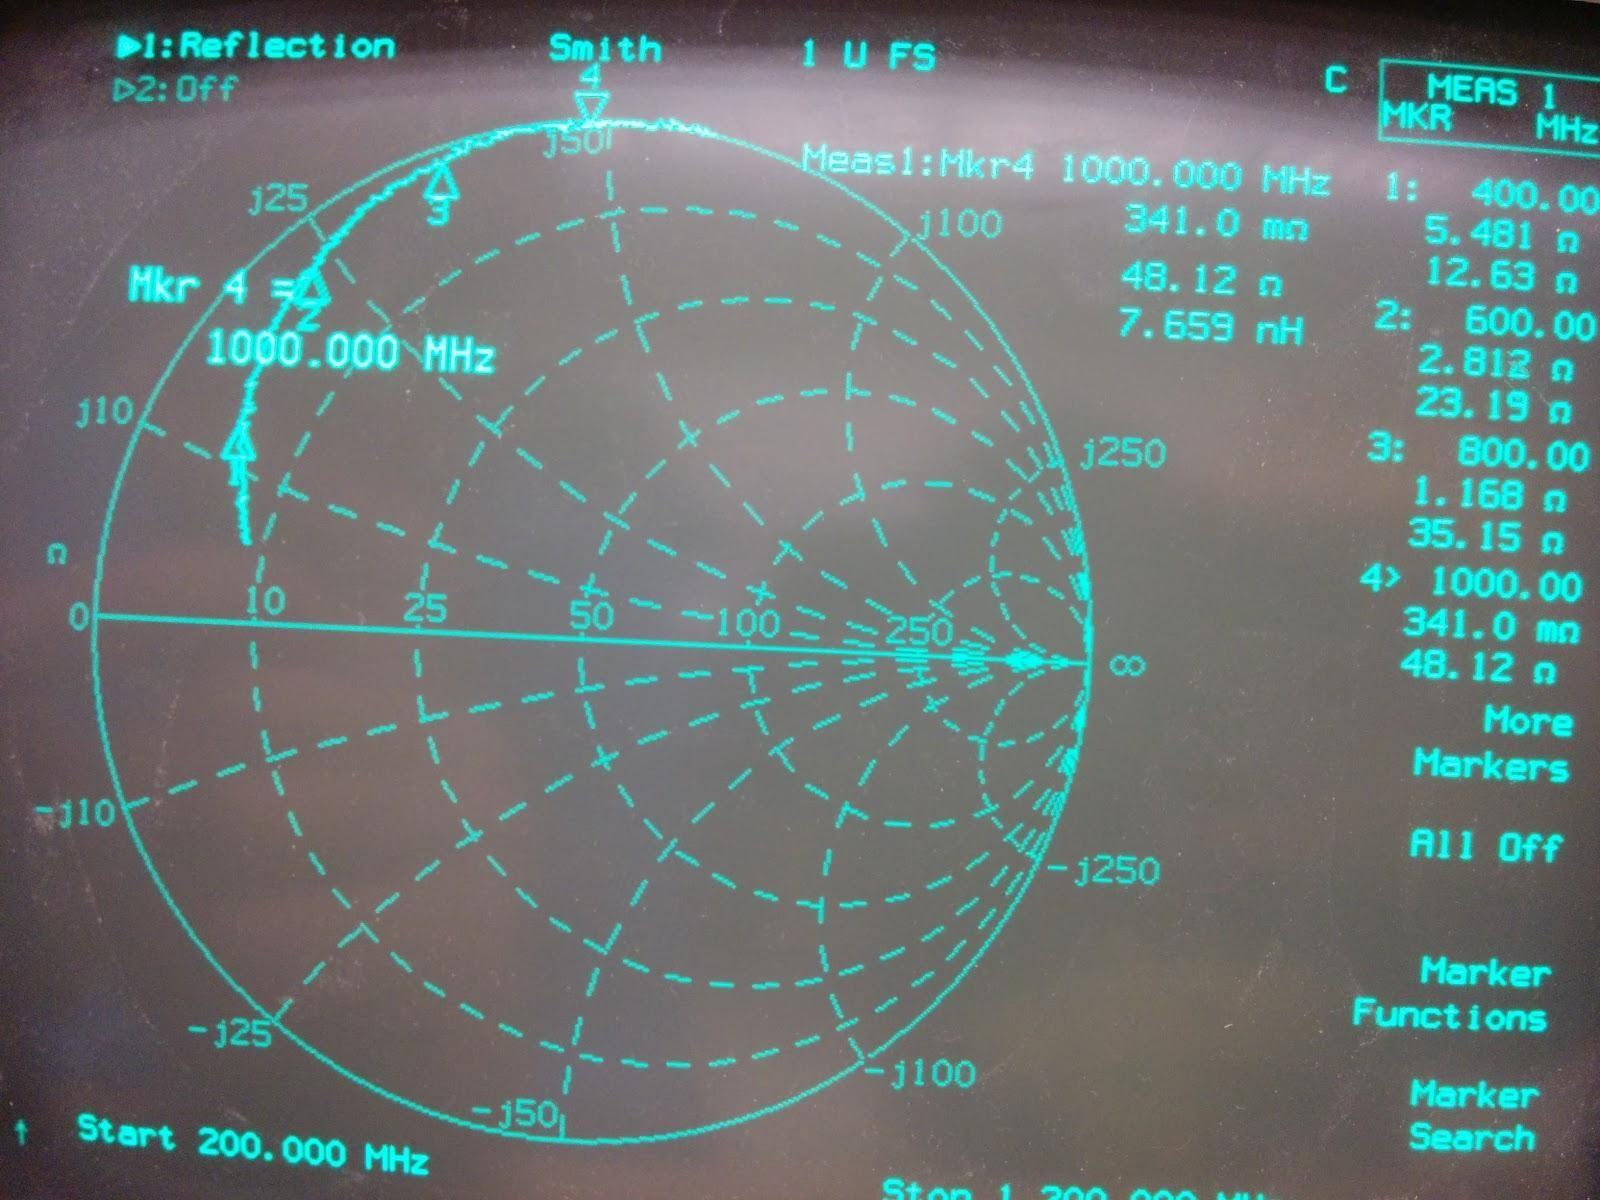
\includegraphics[width=0.8\textwidth]{./Images/253parallel.jpg}
    \caption{Network Analyzer response for a parallel load}
\end{figure}
\begin{figure}[H]
    \centering
    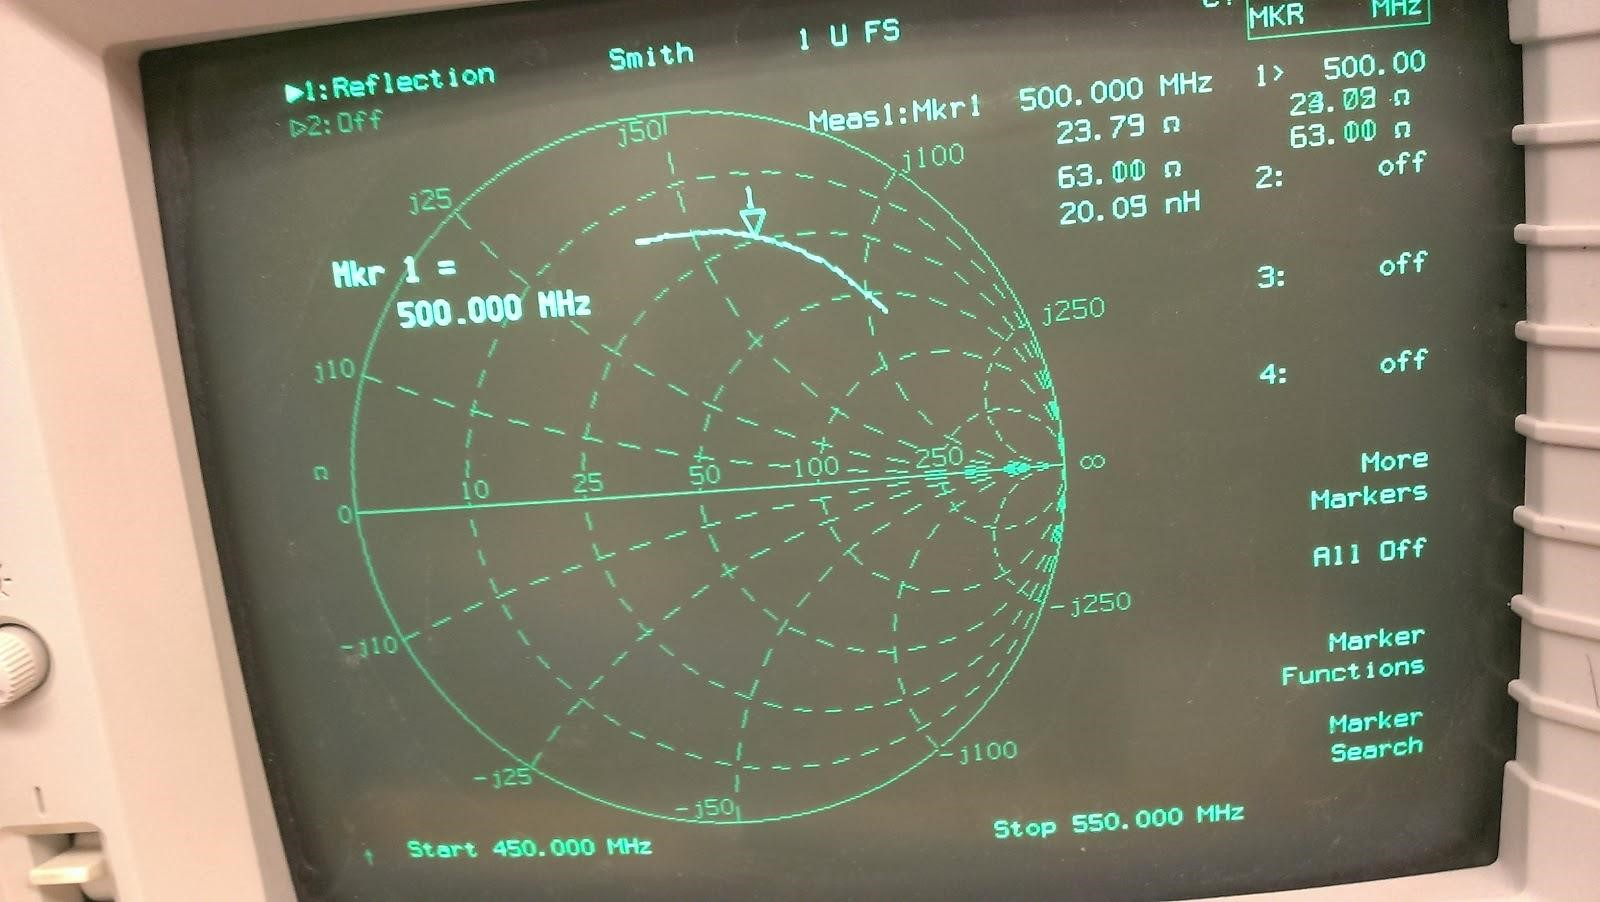
\includegraphics[width=0.8\textwidth]{./Images/254noadj.jpg}
    \caption{Network Analyzer response for the unmatched load}
\end{figure}
\begin{figure}[H]
    \centering
    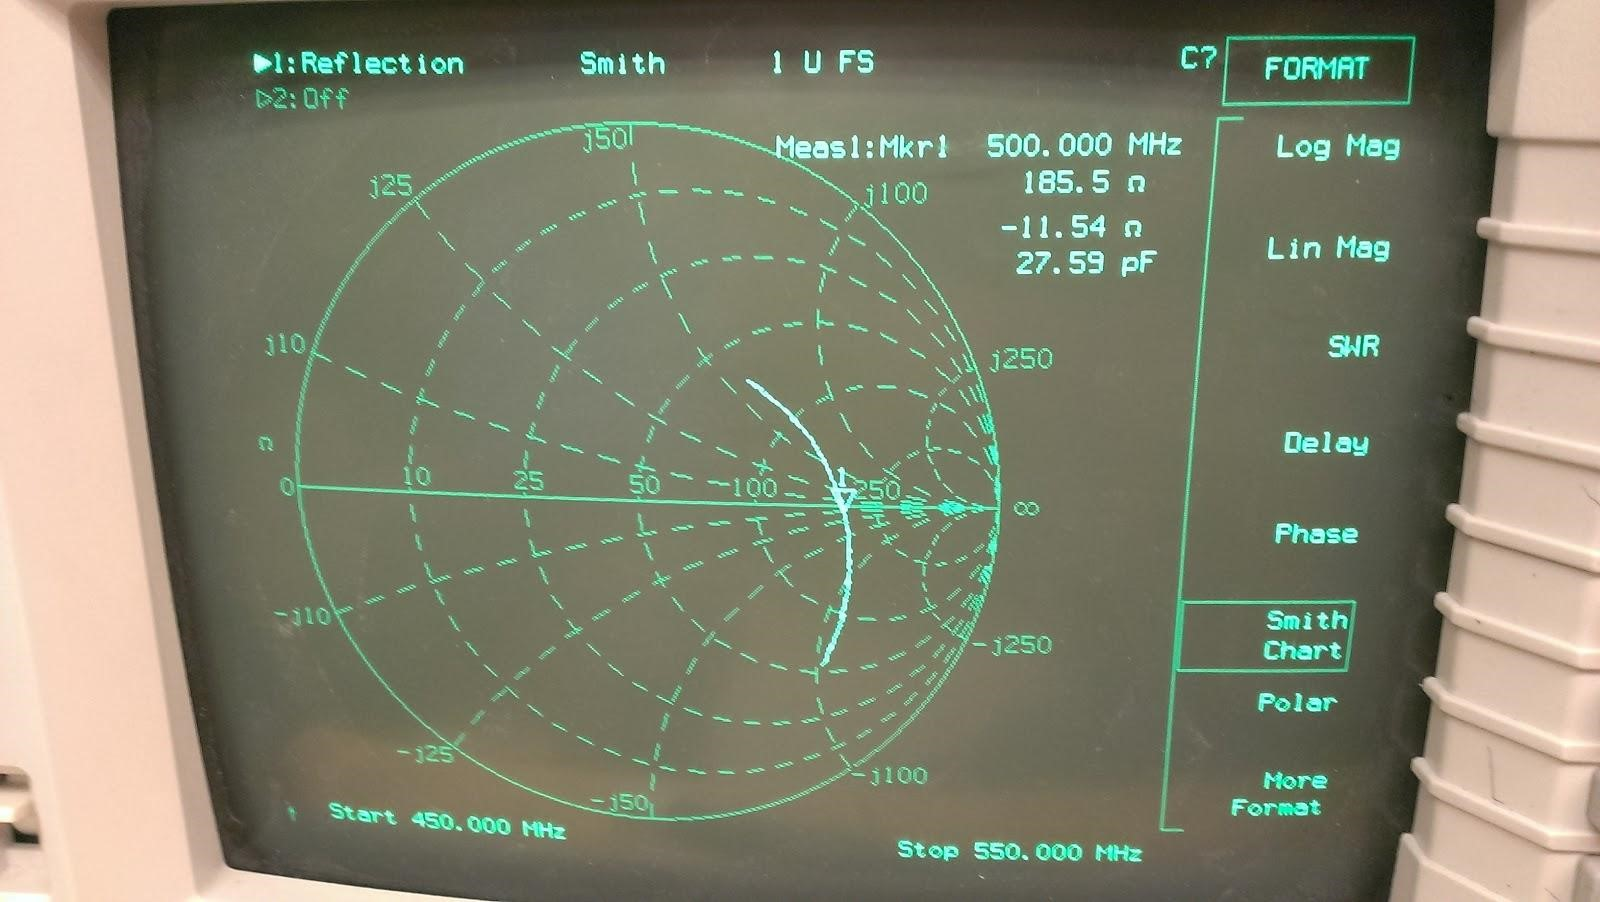
\includegraphics[width=0.8\textwidth]{./Images/254adj.jpg}
    \caption{Network Analyzer response for the matched load with the shorted stub}
\end{figure}
\end{document}